%%%%%%%%%%%%%%%%%%%%%%%%%%%%%%%%%%%%%%%%
%%%%% NATURE CLIMATE CHANGE FORMAT %%%%%
%%%%%%%%%%%%%%%%%%%%%%%%%%%%%%%%%%%%%%%%
%% Comment "% WPcomment" lines, uncomment "% NCCcomment" lines as well as the lines below, replace all citet/citep by cite

% \documentclass{nature}
% \usepackage{amsmath}
% \usepackage{amssymb}
% \usepackage{eurosym}
% % The following allows keeping figures within the text (otherwise nature.cls would ignore them)
% \usepackage{graphicx}
% \makeatletter
% \let\saved@includegraphics\includegraphics
% \AtBeginDocument{\let\includegraphics\saved@includegraphics}
% \renewenvironment*{figure}{\@float{figure}}{\end@float}
% \makeatother

% Nature guidelines (not NCC!)
% Sections can only be used in Articles.  Contributions should be organized in the sequence: title, text, methods, references, Supplementary Information line (if any), acknowledgements, interest declaration, corresponding author line, tables, figure legends.

% No subsubsection nor paragraph

% Spelling must be British English (Oxford English Dictionary)

%Each figure legend should begin with a brief title for the whole figure and continue with a short description of each panel and the symbols used. For contributions with methods sections, legends should not contain any details of methods, or exceed 100 words (fewer than 500 words in total for the whole paper). In contributions without methods sections, legends should be fewer than 300 words (800 words or fewer in total for the whole paper).

% Articles are restricted to 50 references,

% In addition, a cover letter needs to be written with the
% following:
% \begin{enumerate}
%  \item A 100 word or less summary indicating on scientific grounds
% why the paper should be considered for a wide-ranging journal like
% \textsl{Nature} instead of a more narrowly focussed journal.
%  \item A 100 word or less summary aimed at a non-scientific audience,
% written at the level of a national newspaper.  It may be used for
% \textsl{Nature}'s press release or other general publicity.
%  \item The cover letter should state clearly what is included as the
% submission, including number of figures, supporting manuscripts
% and any Supplementary Information (specifying number of items and
% format).
%  \item The cover letter should also state the number of
% words of text in the paper; the number of figures and parts of
% figures (for example, 4 figures, comprising 16 separate panels in
% total); a rough estimate of the desired final size of figures in
% terms of number of pages; and a full current postal address,
% telephone and fax numbers, and current e-mail address.
% \end{enumerate}

% See \textsl{Nature}'s website
% (\texttt{http://www.nature.com/nature/submit/gta/index.html}) for
% complete submission guidelines.

%%%%%%%%%%%%%%%%%%%%%%%%%%%%%%%%
%%%%% WORKING PAPER FORMAT %%%%%
%%%%%%%%%%%%%%%%%%%%%%%%%%%%%%%%
%% Comment "% NCCcomment" lines, uncomment "% WPcomment" lines as well as the lines below
\documentclass[12pt,english]{article}
\usepackage[utf8]{inputenc}
\usepackage{tgpagella} % Palatino text only
\usepackage{mathpazo}  % Palatino math & text
\usepackage[left=1.5in,right=1.5in,top=1.5in,bottom=1.5in]{geometry}
% \linespread{1.5}
\usepackage{bm}
\usepackage{indentfirst}
\usepackage[hyphens]{url}
\usepackage{hyperref}
\hypersetup{
  colorlinks=true, % breaklinks=true,
  urlcolor=purple,    % color of external links
  linkcolor=blue,  % color of toc, list of figs etc.
  citecolor=violet,   % color of links to bibliography
}
\usepackage[hyperpageref]{backref} % back references biblio
\usepackage{tocbibind}
\usepackage[super,comma,sort]{natbib}
% \usepackage[round,sort&compress]{natbib}
\setcitestyle{aysep={}} 
\usepackage{amsmath}
\usepackage{amssymb}
\usepackage{eurosym}
\usepackage{amsfonts}
\usepackage{enumerate}
\usepackage{babel}
\usepackage{caption}
\usepackage{supertabular}
\usepackage{tabularx}
\usepackage{float}
\usepackage{dsfont}
\usepackage{fancyvrb}
\usepackage{verbatim}
\usepackage{enumitem}
\usepackage{setspace}
\usepackage{comment}
\usepackage{subcaption}
\usepackage{graphicx}
\usepackage{tikz}
\usepackage{gensymb}
\usepackage{textcomp}

\usepackage{tabulary}
\usepackage{tabularx}
\usepackage{booktabs}
\usepackage{fullpage}
\usepackage{morefloats}
\usepackage{makecell}
\usepackage{lscape}
\usepackage{pdflscape}
\usepackage{longtable}
\usepackage{rotating}
\usepackage{fancyhdr}
\usepackage{tocloft}
\usepackage{multibib}
\usepackage{titletoc}
\usepackage[export]{adjustbox}
\usepackage[anythingbreaks]{breakurl} % for links
%\usepackage[nomarkers,figuresonly]{endfloat} % Figures at the end
%\usepackage[section,below]{placeins} % Floats placed in the section they appear in.

% % Getting landscape page and page number/footer on bottom of page (instead of to the left)
% \fancypagestyle{mylandscape}{
% \fancyhf{} %Clears the header/footer
% \fancyfoot{% Footer
% \makebox[\textwidth][r]{% Right
%   \rlap{\hspace{1.5cm}% Push out of margin by \footskip
%     \smash{% Remove vertical height
%       \raisebox{13.6cm}{% Raise vertically
%         \rotatebox{90}{\thepage}}}}}}% Rotate counter-clockwise
% \renewcommand{\headrulewidth}{0pt}% No header rule
% \renewcommand{\footrulewidth}{0pt}% No footer rule
% }

% \fancypagestyle{page_left}{%
% 	\renewcommand{\headrulewidth}{0pt}
%   \fancyhf{}
%   \fancyfoot[OC]{%
%       \begin{tikzpicture}[remember picture,overlay]
%           \node[xshift=1cm] (number) at (current page.west) {\thepage};
%       \end{tikzpicture}
%   }%
% }
% \renewcommand{\thesubfigure}{\Alph{subfigure}}

% \newcites{App}{Appendix References}

% \captionsetup[table]{skip=-10pt}
% \begin{document}

% \maketitle

% \clearpage
% % \startcontents
% % \printcontents{ }{1}{\section{\contentsname}}
% % \clearpage
% \section{Introduction\label{sec:intro}}

% % \clearpage
% \renewcommand{\bibsection}{\section{\refname}}
% \bibliographystyle{naturemag}
% \bibliography{global_tax_attitudes}
% % \stopcontents

% \end{document}


\title{International Attitudes Toward Global Policies %\\ Addressing Climate Change and Inequality 
} 

\author{Adrien Fabre$^{1,2}$, Thomas Douenne$^3$ and Linus Mattauch$^4$} % WPcomment
\author{Adrien Fabre\footnote{CNRS, CIRED. E-mail: fabre.adri1@gmail.com (corresponding author).}, Thomas Douenne\footnote{University of Amsterdam}\; and Linus Mattauch\footnote{TU Berlin}~~\thanks{The project %is approved by IRB at Harvard University (IRB21-0137), and 
was preregistered in the Open Science Foundation registry (\href{https://osf.io/fy6gd}{osf.io/fy6gd}). \\ We are grateful for financial support from the University of Amsterdam and TU Berlin. %We are grateful for financial support from the OECD, the French Ministry of Foreign Affairs, the French Conseil d’Analyse Economique and the Spanish Ministry for the Ecological Transition and Demographic Challenge. We also acknowledge support from the Grantham Foundation for the Protection of the Environment and the Economic and Social Research Council through the Centre for Climate Change Economics and Policy. 
We thank Antoine Dechezleprêtre, Tobias Kruse, Bluebery Planterose, Ana Sanchez Chico, and Stefanie Stantcheva for their invaluable inputs for the project. We thank Auriane Meilland for feedback. We thank Laura Schepp, Martín Fernández-Sánchez, Samuel Gervais, Samuel Haddad, and Guadalupe Manzo for assistance in the translation. }} % NCCcomment

\date{\today} % NCCcomment

\begin{document}

\maketitle

\begin{center}
{\textbf{\href{https://github.com/bixiou/global_tax_attitudes/raw/main/paper/US1.pdf}{Link to most recent version}}}
\end{center}


% WPcomment
% \begin{affiliations}
% \item CNRS
% \item CIRED
% \item University of Amsterdam
% \item TU Berlin
% \end{affiliations}

% \begin{small} % NCCcomment
\begin{abstract} % 250 words. TODO? mention more the other measures?
  The ``Global climate scheme'' (a global carbon price funding a global basic income) would be an effective and progressive way to combat climate change and poverty. Yet, such policy is mostly absent from political platforms and the policy debate. Using surveys on 40,000 respondents in 20 countries covering 72\% of global CO$_\text{2}$ emissions, we document majority support for this and other global policies. Using a complementary survey on 3,000 U.S. respondents,% and four European countries, 
  we test several hypotheses that could reconcile strong stated support with a lack of salience of these issues. The complementary analyses show that the stated support is mostly sincere, although we cannot rule out insincerity for 3\% to 9\% of the population from the willingness to sign a real-stake petition and a list experiment, respectively. Global redistributive policies rank high (though not highest) in the prioritization of policies. Conjoint analyses reveal that the Democratic party would not significantly lose votes if it endorsed the global climate scheme, while a candidate at the Democratic primary would actually win votes by doing so. Accurate beliefs about the level of support for the scheme dismisses the hypothesis of pluralistic ignorance of the support. Strong universalistic attitudes are confirmed in more general questions, suggesting that the support cannot be explained away by malleable opinion or experimenter demand. Finally, we conclude that there is no compelling reason why global policies do not enter the public debate or political platforms, as they seem genuinely supported by a majority of the population.
\end{abstract}
% \end{small} % NCCcomment
% TODO!! Methods, Annex, update figures, reduce size

\textbf{JEL codes:} P48, Q58, H23, Q54 % NCCcomment
% Q54 Climate • Natural Disasters and Their Management • Global Warming
% Q58 Government Policy (Q is Environmental econ)
% D78 Positive Analysis of Policy Formulation and Implementation
% H23 Externalities • Redistributive Effects • Environmental Taxes and Subsidies (H is public econ)
% P48 Political Economy • Legal Institutions • Property Rights • Natural Resources • Energy • Environment • Regional Studies (P4 is Other economic systems)
% H41 Public Goods
% H54 Infrastructures • Other Public Investment and Capital Stock

\textbf{Keywords:} Climate change, global policies, cap-and-trade, perceptions, survey.%, inequality, wealth tax. % NCCcomment

\onehalfspacing % NCCcomment

\section{Introduction}  % NCCcomment
% TODO change the intro, e.g. Global poverty and climate change are among the most critical issues faced by the world today", and then explain that the first could be solved by transfer, the second by capping pollution, hence an effective policy to tackle these two problems is the GCS. Yet, this policy is nowhere to be seen in policy debates. Why? In this paper we provide evidence from surveys showing that people all over the world support this policy. To explain this paradox (people stated support vs absence of the policy), we further investigate the sincerity of these claims and rationales behind the support, etc.
Ethical theories often warrant transfers from high- to low-income people, hence from high- to low-income countries. This is the case of utilitarianism, the benchmark ethical theory used in economics. Utilitarianism assigns the same weight to each person and thus considers that a dollar is better allocated to a low-income person, which has a higher marginal utility than a high-income person.\cite{mill_utilitarianism_1861} 

Addressing global poverty, inequalities and climate change are at the heart of the universally agreed Sustainable Development Goals (SDG). % 12 out of  17
It has been pointed out that low-income countries generally do not have enough domestic resources to eliminate the poverty gap in the short run.\cite{bolch_arithmetics_2022} In other words, it would hardly be possible to achieve the first SDG and end extreme poverty by 2030 without international transfers. 

Climate change is another issue that calls for a global response and in particular international transfers. Postulating %Assuming
that each human has an equal right to emit CO$_\text{2}$, low emitters have a legitimate claim \textit{vis-à-vis} high emitters, that can be settled by monetary transfers. Coupling this burden-sharing principle to the carbon budget (remaining emissions that would be compatible with the Paris agreement) naturally defines a global climate policy. We call it the ``Global climate scheme'' (GCS); it consists of a global cap-and-trade system where emission rights are auctioned each year to polluting firms and the revenues finance a global basic income. Using the price and emissions trajectories from the Stern-Stiglitz report,\cite{stern_report_2017} we estimate that the basic income would amount to \$30 per month for each human above 15 in 2030, enough to lift out of extreme poverty the 700 million people who live with less than PPP \$2 per day. Conversely, high emitters like a typical American (with median U.S. CO$_\text{2}$ emissions) would lose in net \$85 per month, as they would face \$115 per month in price increases (assuming a carbon price of \$90/tCO$_\text{2}$ in 2030). % TODO Give the numbers in the Results section
% G default policy for economists, we focus on it; transfers at heart of COP; global wealth tax proposed by Piketty, Saez (fair and effective); democratisation of int'l institutions recurring topic.
% Few studies on CC burden-sharing, all compatible with G
% Few studies on global policies, but they show support (Ghassim, Carattini 19)
% Here, two sets of results. First, twenty countries. Second, dig deeper using complementary survey.

If high emitters share universalistic ethical values, we expect strong support for the GCS, even in high-income countries. On the contrary, if people defend their own financial interest, we expect low support for the GCS in high-income countries. 

In this paper, we study attitudes toward global policies that address climate change, global poverty or inequalities, with a focus on the GCS. We measure stated support for different global policies using unpublished % TODO better way to sell these results?
results from a survey\cite{dechezlepretre_fighting_2022} on climate attitudes conducted in 2021 on 40,680 respondents from 20 countries covering 72\% of global CO$_\text{2}$ emissions. We then conduct a representative survey on 3,000 U.S. respondents to study in detail the sincerity and rationales behind the support for the GCS, the attitudes toward various global policies, global redistribution, and universalistic values.

\section{Results}
% TODO short data section
% % 4 most important figures: heatmap OECD, heatmap support, prioritization or conjoint (r), list exp (table)
\subsection{Global support}
The global survey shows strong support for climate policies at the global level (Figure \ref{fig:oecd}). When asked ``At which level(s) do you think public policies to tackle climate change need to be put in place?'', 70\% (in the U.S.) to 94\% (in Japan) choose the global level. Meanwhile, the European level is chosen by less than half of the European respondents while the federal level is chosen by only 52\% of U.S. respondents. More local levels are generally chosen less than broader ones. This preference for the global level is consistent with (at least) two of the three key motives to support climate policies identified in the literature:\cite{klenert_making_2018,douenne_yellow_2022,dechezlepretre_fighting_2022} effectiveness and fairness (the third being self-interest). 

\begin{figure} % TODO have a simpler title (e.g. "Attitudes towards global climate policies"), and a note explaining what the figure exactly does (unit of the numbers, meaning of the colors, exclusion of indifferent people, etc.
  \caption{Share of support (somewhat or strongly) for the main global policies among non-\textit{indifferent} ($n$ = 40,680).} % TODO: add G to this heatmap, remove Dependence on what other countries do, change label titles to make it clear that the first one was multiple answers while the others were likert
  \makebox[\textwidth][c]{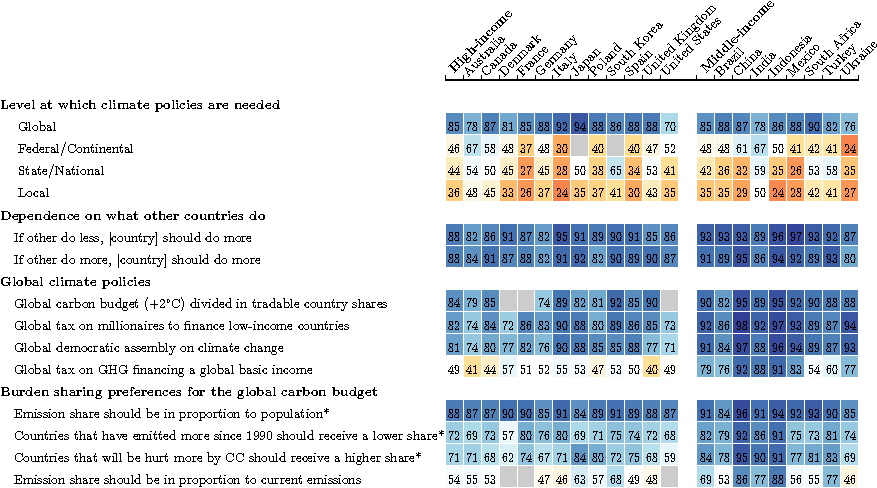
\includegraphics[width=\textwidth]{../figures/OECD/Heatplot_burden_share_all_share_countries.pdf}}\label{fig:oecd}
\end{figure}

Several global policies obtain an absolute majority %more than 70\% relative %
support in all countries: ``a tax on all millionaires in dollars around the world to finance low-income countries that comply with international standards regarding climate action [which] would finance infrastructure and public services such as access to drinking water, healthcare, and education'', % TODO shorten
``a global democratic assembly whose role would be to draft international treaties against climate change [where] each adult across the world would have one vote to elect members of the assembly'' (though this one receives only 48\% of support in the U.S.), and an international emission trading scheme where ``countries that emit more than their national share would pay a fee to countries that emit less than their share''. 
In high-income countries, this global quota obtains 64\% of absolute (i.e. \textit{somewhat} or \textit{strong}) support and 84\% of relative support (i.e. excluding \textit{indifferent} answers). The support is even higher in middle-income countries, though one should interpret the results with caution in middle-income countries as their samples are only representative of the online population (young, graduated and urban people are over-represented). % TODO: not asked this way in FR, DK, US: comment
After the support for the global quota, we ask how the carbon budget should be divided among countries. 
The preferred burden-sharing rule is to allocate the rights to emit on an equal per capita basis: this fairness principle secures an absolute majority support in all countries, and a relative majority support never below 84\%. 
Taking into account historical responsibilities and vulnerability to climate damages is also popular, though less consensual, while grand-fathering (i.e. allocating emission shares in proportion to current emissions) comes last everywhere. 
The Global climate scheme, i.e. a global quota where emission rights are allocated on an equal per capita basis, has the same distributive effects as a global carbon tax that would fund a global basic income. We also test the support for this policy, but here we specify to the respondents the distributive effects: that it would lift the 700 million people who earn less than \$2/day out of extreme poverty, and that the typical person in their country would lose a certain amount (that we specify) due to the price increases.  % The average British person would lose a bit from this policy as they would face £42 per month in price increases, which is higher that the £22 they would receive.
Despite their similarity, the global tax is less supported than the global quota, and it even fails to obtain a majority in Anglo-saxon countries. This lower support is likely due to the fact that distributive effects are made salient in the case of the tax, an interpretation that is consistent with the level of support for the global quota once we make the distributive effects salient, which we do in the complementary surveys. % though we cannot exclude that people find a quota more effective than a tax to reduce emissions. 


\subsection{Stated support for various policies}
% H0: Majority support for each global policies except maximum wealth and debt cancellation

\subsubsection{Global climate scheme} % NCCcomment
In the complementary U.S. survey, we describe the Global climate scheme, explain its distributive effects (specifying the amounts at stake), test the understanding that typical people would lose in high-income countries and that the poorest humans would win using an incentivized question, and then give the correct answer. We proceed the same way for a National redistribution scheme (NR) that would tax the top 5\% to finance cash transfers offseting the monetary loss of the GCS for the median emitter, expecting people to find out at the comprehension question that the richest would lose and the typical people in their country would win. Then, we display summaries of the schemes' description to make sure that the respondents remember them. Right after, we ask again incentivized question of comprehension, and latter give the expected answer that a typical fellow citizen would neither win nor lose with the GCS and NR combined. Finally, we directly ask the support for the GCS and for NR in simple \textit{Yes}/\textit{No}: the stated support for each is at 54\% ($n$ = 3,000).% TODO add something if equality remains

\subsubsection{Other global policies} % NCCcomment
We also test support for other %more realistic
global policies (Figure \ref{fig:support}). All receive relative majority support but two: ``a maximum wealth limit of \$10 billion'' and the ``cancellation of low-income countries' public debt''. Climate-related policies are particularly popular: ``high-income countries funding renewable energy in low-income countries'' obtains absolute majority support while loss and damages compensation (which was approved at the COP27) receives a relative support of  57\%. 

\begin{figure}
  \caption{Support for various global policies in the U.S. ($n$ = 3,000).}
  \makebox[\textwidth][c]{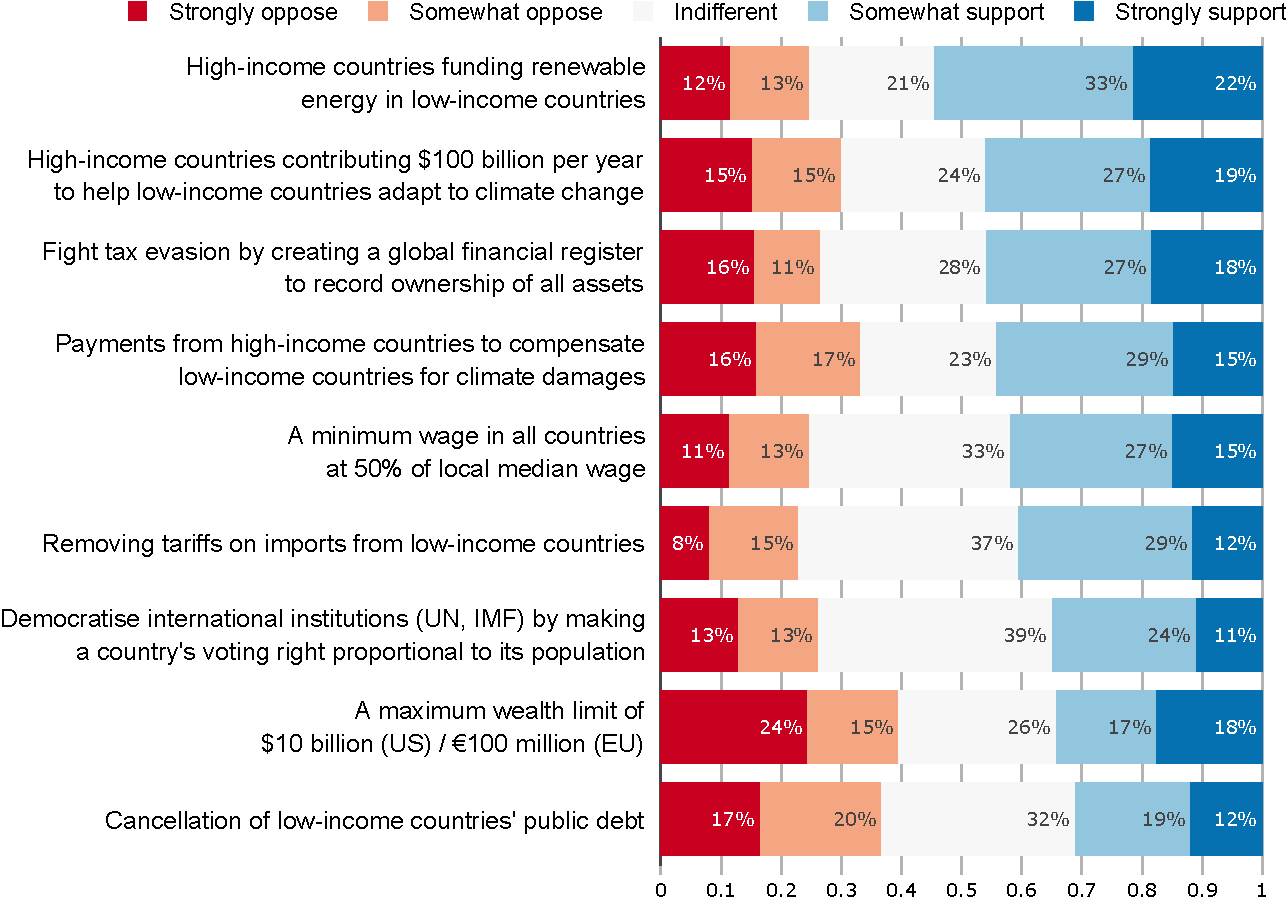
\includegraphics[width=\textwidth]{../figures/US1/support_likert.pdf}}\label{fig:support}
\end{figure}

% H0: Foreign aid: less than 20\% want a decrease (because nationalist), median wants increase at some conditions (no diversion, human rights) => GCS mostly addresses these points
\subsubsection{Foreign aid} % NCCcomment
After explaining that ``0.4\% of U.S. government spending (that is, 0.2\% of U.S. GDP) is spent on foreign aid to reduce poverty in low-income countries'', less than 20\% state that U.S. foreign aid should be reduced while 57\% state that it should be increased, including 14\% who support an unconditional increase. To the 43\% who answer that aid should be increased but only if some conditions are respected, we later ask them what condition(s) should be required. The three conditions most chosen are all largely respected by the Global climate scheme: ``that we can be sure the aid reaches people in need and money is not diverted'' (chosen by 74\%), ``that recipient countries comply with climate targets and human rights'' (59\%), and ``that other high-income countries also increase their foreign aid'' (44\%). %, we propose different conditions. The most chosen condition (by 74\%) is  and the second most (by 59\%) ``That recipient countries comply with climate targets and human rights''. 
On the other side, not wishing to increase their country's foreign aid is mostly justified by prioritizing one's fellow citizens or viewing each country as responsible for its own fate. 

\subsection{Sincerity of support}

We use several methods to assess the sincerity of the support for the Global climate scheme: a list experiment, a real-stake petition, conjoint analyses, and the prioritization of policies. All methods suggest that the support is either completely sincere, or the share of insincere answers is limited. 

\subsubsection{List experiment}  % NCCcomment
% H1: List experiment: There seems to be a 8pp social norm (differential of 3pp with NR). No effect of the number of options. TODO: check literature
The tacit support for the GCS measured through the list experiment is 46\%, i.e. 8 p.p. lower than at the direct question. This may be the sign of a social norm pushing some people to state that they support the GCS although they secretly do not. Still, if there is a social norm in favor of the GCS, there is a similar norm in favor of the National redistribution scheme, as the gap between the tacit and direct support for it is comparable (at 7 p.p.). %However, two observations qualify this interpretation. First, the gap between the tacit and direct support for the National redistribution scheme is comparable (at 7 p.p.) though we did not expect such a social norm in the case of the national redistribution, as the 95\% who would benefit from it should not feel ashamed to oppose a policy that would benefit them. Second, while we tested the questionnaire on random people in cafés, we noticed that some were confused by the question of the list experiment (asking how many policies from the list they supported), upset with the conservative societal policy (``Marriage only for opposite-sex couples in the U.S.'', ``Death penalty for major crimes'' in Europe), to the point that they did not answer attentively.

\begin{table}\label{tab:list_exp}
  \caption{Number of supported policies in the list experiment in function of the composition of the list. $G$ stands for the Global climate scheme and $R$ for the National redistribution scheme ($n$ = 3,000).} % Beware, this question is quite unusual. \\ Among the policies below, how many do you support?  \\ Coal exit, Marriage only for opposite-sex couples 
  \makebox[\textwidth][c]{
\begin{tabular}{@{\extracolsep{5pt}}lc} 
\\[-1.8ex]\hline 
\hline \\[-1.8ex] 
\\[-1.8ex] & Number of supported policies \\ 
\hline \\[-1.8ex] 
Mean & 1.364  \\ \hline \\[-1.8ex]
 List contains: G & 0.464$^{***}$ \\ 
  & (0.054) \\ 
  List contains: R & 0.494$^{***}$ \\ 
  & (0.053) \\ 
  List contains: G $\times$ R & $-$0.001 \\ 
  & (0.091) \\ 
 \hline \\[-1.8ex] 

Observations & 1,799 \\ 
R$^{2}$ & 0.111 \\ 
\hline 
\hline \\[-1.8ex] 
\end{tabular} }
\end{table}

% Donation addresses experimenter demand
\subsubsection{Petition} % Addresses hypothetical bias  % NCCcomment
% H1: Petition: Small effect against GCS: -4pp
When told that ``we will send the results to the U.S. President's office, informing him what share of American people are willing to endorse the Global climate scheme'', 4 p.p. fewer people are willing to sign a petition for the GCS than to simply state their support. For the National redistribution scheme, the proportion of support is not significantly different in the petition and in the simple question. 

\subsubsection{Conjoint analyses} % Addresses acquiescence bias  % NCCcomment
% H1, H2: Conjoint analysis: G|C+R 56%, G|R 59%, G 48% ~ C (|R), G+C|R 56%, C|R 64%, Left+G - Left = -3pp, A+G vs. B 59%
% => G is supported for itself, rather independently from R or C, with similar support to both, and it doesn't significantly penalize the Left, and would help a Democratic candidate
In our \textit{conjoint analyses}, we ask respondents to make five choices between pairs of political platforms. The first conjoint analysis suggests that the GCS is supported for itself, independently from being complemented by a national climate policy (``Coal exit''% in the U.S., ``Thermal insulation plan'' in Europe
, denoted C) and the National redistribution scheme. Indeed, 55\% of ($n$ = 3,000) respondents prefer the combination of C, NR and the GCS to the combination of C and NR alone, indicating a similar support for the GCS conditional on NR and C than for the GCS alone (as it does not significantly differ from the direct support of 53\%). For the second analysis, we split the sample into four random branches. This analysis shows that the preference for C, NR and the GCS together is as high, at 55\% ($n$ = 750), if the alternative is NR alone; that the support for the GCS conditional on NR, at 59\% ($n$ = 750), is somewhat higher than the direct support for the GCS; that the support for C conditional on NR is even higher, at 63\% ($n$ = 750); which is confirmed by the fact that 52\% ($n$ = 750) prefer C to the GCS (both) conditional on NR. In other words, there is majority support for the GCS and for C, slightly more people prefer C but C does not act as a substitute for the GCS, and some people find the GCS complementary to NR though the number of people requiring NR to support the GCS remains small. % TODO rework this paragraph

The third analysis suggests that a Democratic candidate would not significantly lose voting share at the 2024 presidential election if he or she were to endorse the GCS. To estimate this, we present to two random branches of the sample hypothetical Democratic and Republican platforms that differ only by the presence (or not) of the GCS in the Democratic platform. Although the share of respondents choosing ``None of them'' is slightly higher (at 13\% instead of 11\%) when the Democratic platform includes the GCS, the share choosing the Democrat is not significantly lower (52\% in both cases). 

Our last two analyses is run on the subsample of non-Republicans ($n$ = 2,000), i.e. the respondents who choose \textit{Democrat}, \textit{Independent}, \textit{Non-Affiliated} or \textit{Other} for their political affiliation. We frame the choice between two platforms as a hypothetical duel at the 2024 Democratic primary and force the respondents to choose between candidate A or B. In the fourth analysis, a policy (or an absence of policy) is randomly drawn for each platform in each of five categories: \textit{economic issues}, \textit{societal issues}, \textit{climate policy}, \textit{tax system}, \textit{foreign policy} (Figure \ref{fig:ca_r}). Except for the category \textit{foreign policy}, which features the GCS 42\% of the time, the policies are prominent progressive policies and they are drawn uniformly. % TODO: check
When a platform features the GCS and not the other, the one with the GCS is chosen 53\% (which is significantly more than half) of the time ($n$ = 3,000). % TODO: effect vis-à-vis baseline (cf. figure)
The fifth analysis draws random Democratic platforms in a similar ways, except that candidate A's platform always contains the GCS while candidate B includes no foreign policy. In this case, 61\% of respondents choose A ($n$ = 3,000). In short, our conjoint analyses indicate that a candidate at the Democratic primary would have more chances to obtain the nomination by endorsing the GCS, and this endorsement would not penalize her or him at the presidential election. % TODO! cite Ghassim

\begin{figure}
  % Imagine that at the 2024 Democratic party presidential primaries, the two main candidates campaign with the following key policies in their platforms. \\ Which of these candidates do you prefer?

  \caption{Conjoint analysis (asked only to non-Republicans). Average Marginal Component Effects (relative to the baseline: an absence of policy of that category) of policies in the choice of candidate for a hypothetical duel in the 2024 Democratic primary, where both platforms are randomly drawn ($n$ = 2,000).}\label{fig:ca_r}
  \makebox[\textwidth][c]{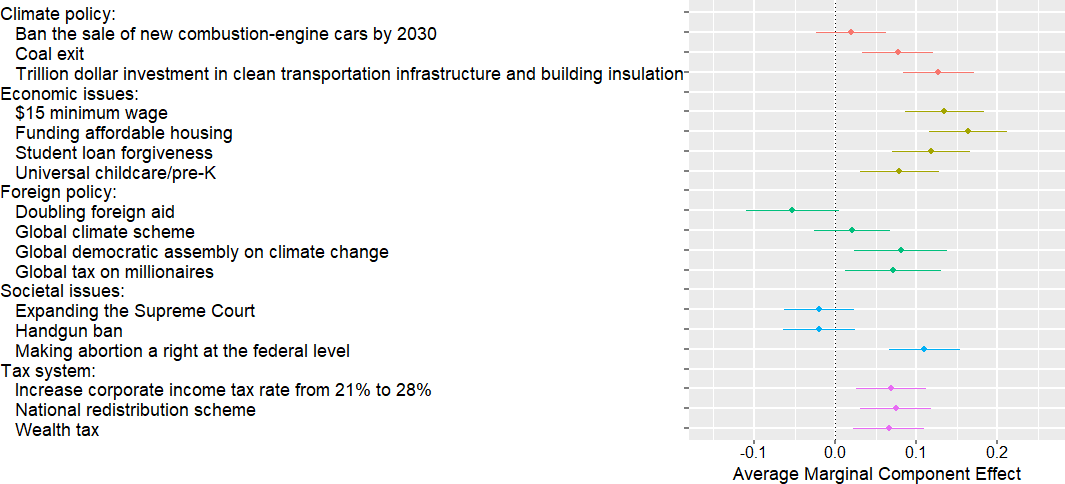
\includegraphics[width=\textwidth]{../figures/US1/ca_r.png}}
\end{figure}

%\subsubsection{Prioritization} % Addresses acquiescence bias and social desirability bias
% H1: Prioritization: G has mean only slightly lower than average, makes better than ban of cars and coal exit; global tax on millionaires does as well as wealth tax and almost as good as $15 minimum wage
At the end of the survey, we pick six policies at random (and uniformly) among the progressive policies used in the last conjoint analyses, and ask respondents to allocate 100 points (using sliders) among them, with the instruction that ``the more you give points to a policy, the more you support it''. For each policy presented, the average support is thus 16.67 points (Figure \ref{fig:points}). The GCS ranks in the middle of all policies (9th. out of 17), with an average number of points of 15.3 which is only slightly lower than average. It is higher than to ``ban the sale of new combustion-engine cars by 2030'' (13.4) and ``coal exit'' (10.0), but lower than the third climate policy: ``trillion dollar investment in clean transportation infrastructure and building insulation'' (20.3). The support for other globally redistributive policies is variable: ``Doubling foreign aid'' is the least supported policy (8.4), while the ``Global tax on millionaires'' is one of the five policies with more than 20 points (20.2), and the ``global democratic assembly on climate change'' is just below the GCS (14.5). The most supported policies are ``Funding affordable housing'' (28.5), ``\$15 minimum wage'' (23.8), and ``Universal childcare/pre-K'' (22.1). % TODO share that allocated at least 1

\begin{figure}
  \caption{Prioritization of policies. Each respondent faces six policies taken at random from the ones below and allocates 100 points among them to signal the strength of their support for each one ($n$ = 3,000).} % Imagine you have 100 points that you can allocate to different policies. The more you give points to a policy, the more you support it.  \\  How do you allocate the points among the following policies?  
  
  \makebox[\textwidth][c]{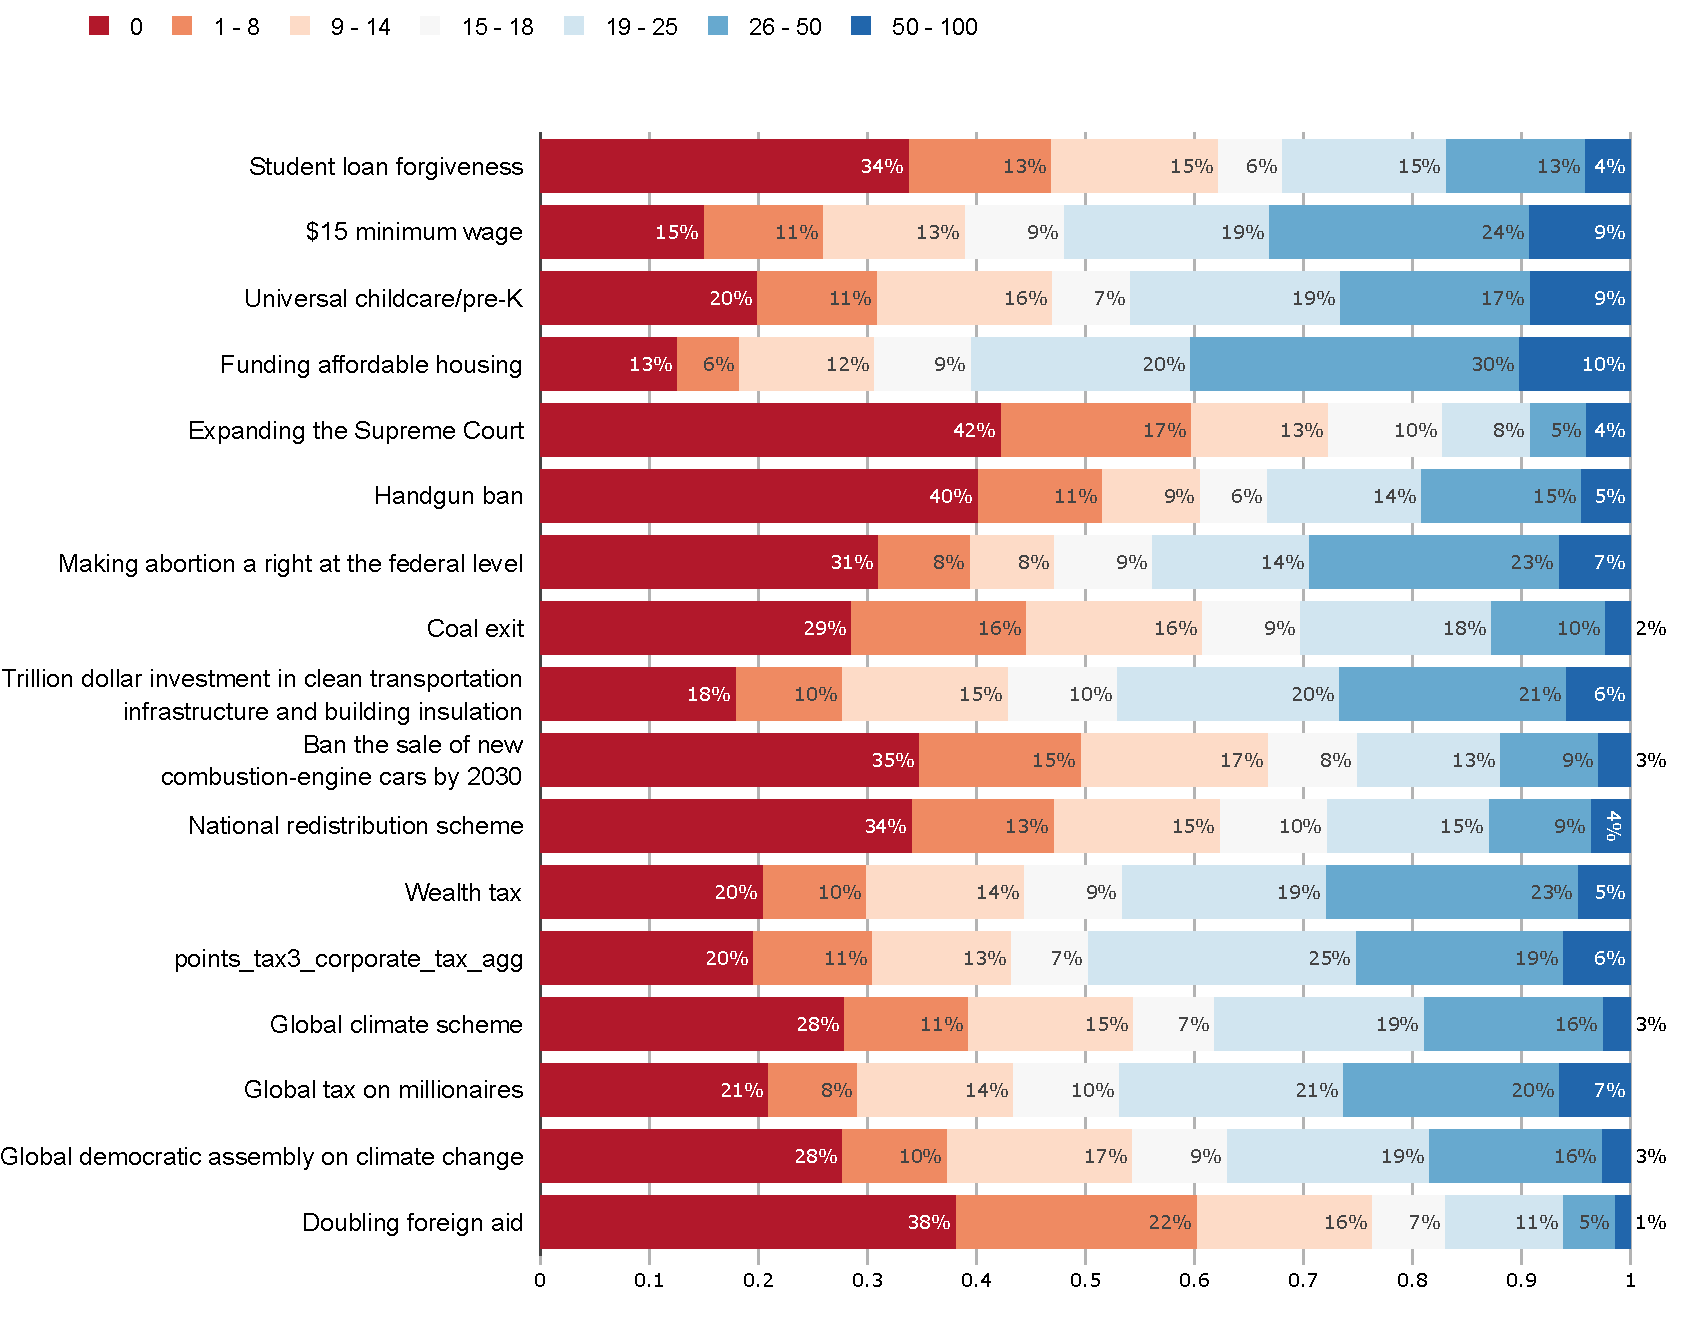
\includegraphics[width=\textwidth]{../figures/US1/points_us.pdf}}\label{fig:points}
\end{figure}


\subsection{Second-order beliefs}
% H3 belief: No pluralistic ignorance
To explain a strong support for the GCS despite its absence from political platforms and the public debate, we hypothesized pluralistic ignorance, i.e. that most people and policy-makers wrongly perceive the GCS as unpopular. People would then hide their support for such globally redistributive policies, knowing that advocating for them would be vain. We do not find any evidence of pluralistic ignorance in an incentivized question on the perceived support. On the contrary, people have quite accurate beliefs regarding the level of support for the GCS. Indeed, the mean (resp. quartiles) perceived support is 52.0\% (resp. 36, 53, 69\%, $n$ = 1,500) vs. an actual support of 53\%. For the record, the second-order beliefs are equally accurate for the National redistribution scheme, with mean (resp. quartiles) perceived support of 54.7\% (resp. 40, 55, 71\%, $n$ = 1,500) vs. 56\%.

\subsection{Universalistic values}
% H4: A strong majority is universalist/cosmopolitan (TODO: which word?), even a majority for non-Republican
% TODO It is not obvious how these answers are informative of malleable opinions. So I don't think we should state the hypothesis and sell this as a test.
Another hypothesis to explain the discrepancy between the lack of interest for global policies in the public debate despite a strong stated support is that opinions on the topic are weak and malleable. A way to test this is to ask broad question on people's values, to see whether their core values are consistent with universalism. Asked what group they defend when they vote ($n$ = 3,000), 19\% choose ``sentient beings (humans and animals)'', 25\% ``humans'', 34\% ``Americans'', 15\% ``My family and myself'', and the rest (7\%) choose another group (mostly ``My State or region'' or ``People sharing my culture or religion''). The first two categories can be described as universalist, and they represent close to one out of two people. The share of universalist even constitutes a majority (at 51\%) of non-Republicans. 
When asked what should U.S. diplomats defend in international climate negotiations, only 14\% prefer ``U.S. interests, even if it goes against global justice''; 25\% prefer global justice (mitigated or not by U.S. interests) and the bulk of respondents (37\%) prefer ``U.S. interests, to the extent it respects global justice'' ($n$ = 3,000). 
Finally, when asked to judge the extent to which climate change, global poverty and U.S. inequality are an issue, climate change is generally viewed as the biggest problem (with a mean of 0.40 once we recode answers between $-2$ and $2$), followed by global poverty (0.20) and U.S. inequality (0.19, $n$ = 3,000). 
Overall, answers to these broad value questions are consistent with half of Americans supporting global policies like the GCS, as people find that global issues are among the biggest problems, almost half of them are universalist when they vote, and most of them wish that U.S. diplomats take into account global justice.


\section{Discussion} % Summary, conclusion
% TODO! alternative explanations: ignorance of G itself (supported by open-ended fields), national institutions bias
In 20 among the largest countries, we find strong majority support for global climate policies, even in high-income countries that would financially lose from the globally redistributive policies that we test. The complementary survey in the U.S. confirms these results. For example, there is a strong support for global taxes on the wealthiest, and majority support for our flagship policy, a Global climate scheme that would establish both carbon pricing at the global level through an emission trading system, and a global basic income funded by its revenues. A list experiment and a real-stake petition show that the support for the GCS is mostly sincere. This genuine support is confirmed by the prioritization of this global climate policy above some prominent national climate policies, and consistent with around half of the population holding universalistic (rather than nationalistic or egoistic) values. Moreover, the conjoint analyses reveals that a Democratic candidate should not lose voting shares by endorsing the GCS, and would even win votes at the Democratic primary by doing so. Besides a potential lack of sincerity and weak opinions, we dismiss another hypothesis to explain the scarcity of global policies in the public debate despite a strong support: that people underestimate the support of their fellow citizens. As we ruled out all our pre-registered hypotheses, we now need to formulate new hypotheses.

We see four potential explanations for the scarce mention of globally redistributive policies in the public debate. Among the new hypotheses, the first two are variations of pluralistic ignorance, and the last two represent complementary (rather than substitute) explanations. First, there may be pluralistic ignorance of univeralistic values, of the support for the GCS, or of the electoral advantage of endorsing it \textit{among policy makers}. We intend to test this hypothesis by running a survey on Congress staffers and Members of the European Parliament. Second, there may be a more subtle form of pluralistic ignorance: although people correctly predict what people would answer to a survey question, they may view globally redistributive policies as unrealistic, perhaps because they have never reflected upon the fact that many people across the world hold univeralistic values and are supportive of global solidarity. Third, most people and perhaps even most policy makers may have simply never heard of the GCS, let alone built their political ideas upon it. The ignorance of the GCS itself seems supported by the feedback fields, where the most common answer is a variation upon ``thank you for this interesting, thought-provoking survey''. Fourth, most institutions are national: the largest scale votes take place at the national level, most media target a national audience, most commentators frame their discourse from a national perspective, and relations to foreign countries as conflictual. The prominence of national institutions may create a nationalistic bias in political thoughts, silencing the univeralistic values of people. % TODO! test hypotheses 2 (is G realistic) and 3 (is G new to you?) in US2?
% TODO! find references

In any case, if any (or several) of the remaining hypotheses is confirmed by evidence, we could draw the same conclusion. % TODO But what if they are not? I don't think that would invalidate the conclusion stated below.
There is a strong support for global policies that address climate change and global inequality, even in high-income countries, and the frontier of what is considered politically realistic might soon shift on this issue. Uncovering evidence for this might actually contribute to garner more attention to global policies in the public debate and political platforms. % TODO I don't like this because it sounds a bit like asking editors to publish our work.

% \begin{methods}  % WPcomment
\begin{small} % NCCcomment
%Put methods in here.  If you are going to subsection it, use \subsection commands.  Methods section should be less than 800 words and if it is less than 200 words, it can be incorporated into the main text.
\section{Methods} % NCCcomment
% \subsection{Method subsection.} 
% Incentives

% Here is a description of a specific method used.  Note that the subsection heading ends with a full stop (period) and that the command is \verb|\subsection{}| not \verb|\subsection{}|.

% \end{methods} % WPcomment
\end{small}  % NCCcomment

% \bibliographystyle{naturemag_noURL} % nature class works only with style naturemag or naturemag_noURL, and naturemag bugs if there are certain URLs (like .pdf). Also, nature class only works with \cite, not \citet or \citep.  % WPcomment
\bibliographystyle{plainnatnourl_clean} % NCCcomment
\bibliography{global_tax_attitudes}

% WPcomment
%% Here is the endmatter stuff: Supplementary Info, etc.
%% Use \item's to separate, default label is "Acknowledgements"
% \begin{addendum} % 177 words
%  \item We are grateful for financial support from the University of Amsterdam and TU Berlin. We are grateful for financial support from the OECD, the French Ministry of Foreign Affairs, the French Conseil d’Analyse Economique and the Spanish Ministry for the Ecological Transition and Demographic Challenge. We also acknowledge support from the Grantham Foundation for the Protection of the Environment and the Economic and Social Research Council through the Centre for Climate Change Economics and Policy. We thank Antoine Dechezleprêtre, Tobias Kruse, Bluebery Planterose, Ana Sanchez Chico, and Stefanie Stantcheva for their invaluable inputs for the project. We thank Auriane Meilland for feedback. We thank Laura Schepp, Martín Fernández-Sánchez, Samuel Gervais, Samuel Haddad, and Guadalupe Manzo for assistance in the translation. 
%  \item[Registration] The project %is approved by IRB at Harvard University (IRB21-0137), and 
%  was preregistered in the Open Science Foundation registry (osf.io/fy6gd).
%  \item[Competing Interests] The authors declare that they have no
% competing interests.
% \item[JEL codes] P48, Q58, H23, Q54.
% \item[Keywords] Climate change, global policies, cap-and-trade, perceptions, survey, inequality, wealth tax.
%  \item[Correspondence] Correspondence and requests for materials
% should be addressed to Adrien Fabre~(email: fabre.adri1@gmail.com).
% \end{addendum}

%%
%% TABLES
%%
%% If there are any tables, put them here.
%%

% \begin{table}
% \centering
% \caption{This is a table with scientific results.}
% \medskip
% \begin{tabular}{ccccc}
% \hline
% 1 & 2 & 3 & 4 & 5\\
% \hline
% aaa & bbb & ccc & ddd & eee\\
% aaaa & bbbb & cccc & dddd & eeee\\
% aaaaa & bbbbb & ccccc & ddddd & eeeee\\
% aaaaaa & bbbbbb & cccccc & dddddd & eeeeee\\
% 1.000 & 2.000 & 3.000 & 4.000 & 5.000\\
% \hline
% \end{tabular}
% \end{table}

\end{document}
